\documentclass{article}
\usepackage{amsmath,amssymb,amsthm,latexsym,paralist,url}
\usepackage[margin=1in]{geometry}
\usepackage{tikz}
\usetikzlibrary{arrows,automata}
\usepackage{csquotes}

\theoremstyle{definition}
\newtheorem{problem}{Problem}
\newtheorem*{solution}{Solution}
\newtheorem*{resources}{Resourcefs}


\newcommand{\honor}{\noindent \textbf{Aggie Honor Statement: }On my honor as an Aggie, I have neither
  given nor received any unauthorized aid on any portion of the academic work included in this assignment.
}

 
\newcommand{\checklist}{\noindent\textbf{Checklist:}
Did you...
\begin{compactenum}
\item abide by the Aggie Honor Code?
\item solve all problems?
\item start a new page for each problem?
\item show your work clearly?
\item type your solution?
\item submit a PDF to gradescope?
\end{compactenum}
}

\newcommand{\problemset}[1]{\begin{center}\textbf{Homework #1}\end{center}}
\newcommand{\duedate}[1]{\begin{quote}\textbf{Due: #1} on gradescope (\url{gradescope.com}). \\You must show your work in order to receive credit.\end{quote}}

%%% CONSTANTS
\newcommand{\mysemester}[0]{Spring 2018}
\newcommand{\mysectionnumber}[0]{501,502}
\newcommand{\myname}[0]{Hunter Cleary}
\newcommand{\homeworknumber}[0]{4}

%%% HEADERS & FOOTERS
\usepackage{fancyhdr} % This should be set AFTER setting up the page geometry
\pagestyle{fancy} % options: empty , plain , fancy
\renewcommand{\headrulewidth}{0pt} % customise the layout...
\lhead{CSCE 222-\mysectionnumber}\chead{Homework \homeworknumber}\rhead{\myname}
\lfoot{}\cfoot{\thepage}\rfoot{}

\title{CSCE 222: Discrete Structures for Computing\\Section \mysectionnumber\\\mysemester}
\author{\myname}
\date{}

\begin{document}

\maketitle
\problemset{\homeworknumber}
\duedate{18 February 2017 (Sunday) before 11:59 p.m.}
\bigskip

\honor
\bigskip

\checklist

% PROOFS
\begin{problem} (25 points)\\
Prove: $(P \wedge T) \to (R \vee S), Q \to (U \wedge T), U \to P, \neg S \vdash Q \to R$
\begin{compactenum}
\item First, by assuming $Q$ and showing $R$.
\item Then, without assuming $Q$ (so you must directly show $Q \to R$) and using the Logic Daemon (\url{logic.tamu.edu}) to check your proof.
\end{compactenum}
\end{problem}

\begin{solution}\ \\
\begin{compactenum}
\item \ \\
$  (P&T)->(RvS),Q->(U&T),U->P,~S,Q|-R
    OK  \ \   1          \ \ (1)   \ \ (P&T)->(RvS)   \ \ A         \ \\
    OK  \ \   2          \ \ (2)   \ \ Q->(U&T)       \ \ A         \ \\
    OK  \ \   3          \ \ (3)   \ \ U->P           \ \ A         \ \\
    OK  \ \   4          \ \ (4)   \ \ ~S             \ \ A         \ \\
    OK  \ \   5          \ \ (5)   \ \ Q              \ \ A         \ \\
    OK  \ \   2,5        \ \ (6)   \ \ U&T            \ \ 2,5->E    \ \\
    OK  \ \   2,5        \ \ (7)   \ \ U              \ \ 6&E       \ \\
    OK  \ \   2,5        \ \ (8)   \ \ T              \ \ 6&E       \ \\
    OK  \ \   3,2,5      \ \ (9)   \ \ P              \ \ 3,7->E    \ \\
    OK  \ \   3,2,5      \ \ (10)  \ \ P&T            \ \ 8,9&I     \ \\
    OK  \ \   3,2,5,1    \ \ (11)  \ \ RvS            \ \ 10,1->E   \ \\
    OK  \ \   3,2,5,1,4  \ \ (12)  \ \ R              \ \ 11,4vE    \ \\
$

\qed

\item \textit{Include a \textbf{clear} screen shot of the correct proof checked by the Logic Daemon.}\\
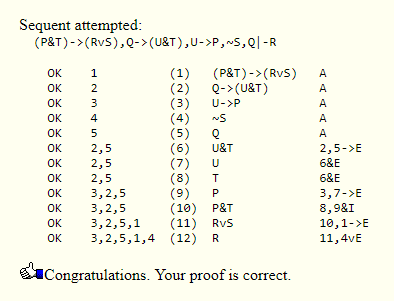
\includegraphics{LogicScreen.png}


\end{compactenum}
\end{solution}

\newpage

% PROOFS
\begin{problem} (25 points)\\
Prove that these 4 statements about the integer $n$ are equivalent:
\begin{compactenum}
\item[(i)] $n^2$ is odd.
\item[(ii)] $1-n$ is even.
\item[(iii)] $n^3$ is odd.
\item[(iv)] $n^2+1$ is even.
\end{compactenum}
\end{problem}

\begin{solution}\ \\
\begin{compactenum}
Showing that $(1) \equiv (2) \equiv (3) \equiv (4)$.\ \\
\ \\
\textit{ k is an integer}\ \\
\ \\
( $(1) \equiv (2)$ )\ \\ 
$n^2$ is odd\ \\
$n*n$ is odd\ \\
n is odd\ \\
$n = 2k + 1$\ \\
$1-n = -2k$\ \\
$\therefore 1-n$ is even\ \\
\ \\ 
( $(2) \equiv (3)$ )\ \\ 
$1-n$ is even\ \\
$1-n = 2k$\ \\
$n = 2k+1$\ \\
n is odd\ \\
$n*n*n$ is odd\ \\
$\therefore n^3$ is odd\ \\
\ \\ 
( $(3) \equiv (4)$ )\ \\ 
$n^3$ is odd\ \\
$n*n*n$ is odd\ \\
$n$ is odd\ \\
$n^2$ is odd\ \\
$n^2 = 2k+1$ \xleftarrow[]{} \text{Add one to both sides}\ \\
$n^2+1 = 2k + 2$\ \\
$n^2+1$ is even\ \\
\ \\
\therefore $(1) \equiv (2) \equiv (3) \equiv (4)$

\end{compactenum}
\end{solution}

\newpage

% PROOFS
\begin{problem} (25 points)\\
Use the notion of "without loss of generality" to prove that
\begin{compactenum}
\item $\min(a,\min(b,c)) = \min(\min(a,b),c)$ when $a,b,c$ are real numbers.
\item $5x+5y$ is an odd integer when $x,y$ are integers of opposite parity\footnote{parity refers to even/odd.}.
\end{compactenum}
\end{problem}

\begin{solution}\ \\
\begin{compactenum}
\item
Assume without loss of generality that $a > b > c$.\ \\
$min(b,c) = c$\ \\
$min(a,c) = c$\ \\
$\therefore \ min(a,min(b,c)) = c$\ \\
$min(min(a,b),c) = c$\ \\
$\therefore \ min(min(a,b),c) = min(a,min(b,c))$
\ \\
\ \\
\text{For every case in which a,b,c are real numbers the solution of the 2 equations will be the same.}
\ \\
\item
Without loss of generality assume that x is even and y is odd.\ \\
$x=2k , y=2k+1$\ \\
k is an integer\ \\
$5x + 5y = 10k + 10k + 5$\ \\
$20k + 5 = $\ \\
$\therefore \ 5x+5y$ is an odd integer. \ \\
In the case where x is odd, y will be even and the same proof will apply.\ \\

\end{compactenum}
\end{solution}

\newpage

% PROOFS
\begin{problem} (25 points)\\
Show that $\sqrt{2} + \sqrt{3}$ is irrational.  You may assume that $\sqrt{n}$ is irrational whenever $n$ is a positive integer that is not a perfect square.
\end{problem}

\begin{solution}\ \\ \ \\
\textbf{Proof by Contradiction}\ \\
Assume that $\sqrt{n}$ is irrational whenever $n$ is a positive integer that is not a perfect square\ \\
Assume that $\sqrt{2} + \sqrt{3}$ is rational.\ \\
$\sqrt{2} + \sqrt{3} = p/q$ (where p and q are integer values)\ \\
$(\sqrt{2} + \sqrt{3})^2 = (p/q)^2$\ \\
$(\sqrt{2}\sqrt{2} +2(\sqrt{3}\sqrt{2}) + \sqrt{3}\sqrt{3})^2 = (p/q)^2$\ \\
$(2 + 2\sqrt{6} + 3) =  (p/q)^2 $\ \\
$(2\sqrt{6} + 5) =  (p/q)^2 $\ \\
$2\sqrt{6} =  (p/q)^2-5$\ \\
$p*p, q*q$ will both be rational numbers (integer times integer)\ \\
Furthermore, an integer value minus an integer value will also be rational.\ \\
$2\sqrt{6} = r/w$ (where r and w are integer values)\ \\
$\sqrt{6} = r/2w$\ \\
$6$ is not a perfect square, $ \sqrt{6}$ is irrational.\ \\
$\therefore \sqrt{2} + \sqrt{3}$ can't be rational and is irrational.
\end{solution}



\end{document}
